\documentclass[]{article}
\pagenumbering{gobble}
\usepackage[a3paper, total={6in, 8in}]{geometry}

\usepackage{pgfplots}
\usepackage{tcolorbox}
\usepackage{circuitikz}
\usepackage{amsmath}
\usepackage{pgfplotstable}
\pgfplotsset{compat=1.18}

\usepackage{tikz}
\usetikzlibrary{automata, positioning, arrows, calc}

\tikzset{
	->,
	>=stealth,
	node distance=3cm,
	every state/.style={thick, fill=gray!10},
	initial text=$ $,
}

\usepackage{tcolorbox}

%opening
\title{Paper assignement 4: TCP message flow charts}
\author{Gabriel PEREIRA DE CARVALHO}
\date{Last modification: \today}

\begin{document}
	
	\maketitle
	
	\section{Scenario 1}
	
	\begin{tcolorbox}
		A client connects to server, server sends data back to client, server closes connection once all data have been sent.
	\end{tcolorbox}
	
	\begin{figure}[h]
		\centering
		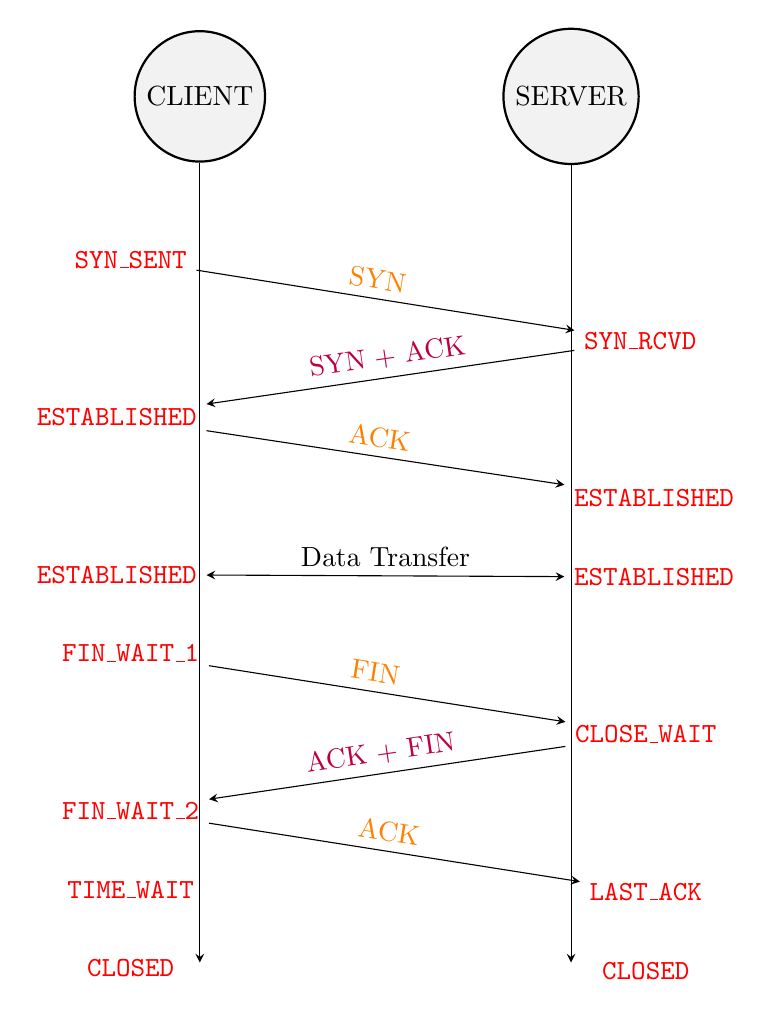
\begin{tikzpicture}
			\node[state] (CLIENT) {CLIENT};
			\node[state, right=of CLIENT] (SERVER) {SERVER};
			\node[below=1cm of CLIENT, xshift=-25] (t0) {\textcolor{red}{$\texttt{SYN\_SENT}$}};
			\node[below=2cm of SERVER, xshift=25] (t1) {\textcolor{red}{$\texttt{SYN\_RCVD}$}};
			\node[below=3cm of CLIENT, xshift=-30] (t2) {\textcolor{red}{$\texttt{ESTABLISHED}$}};
			\node[below=4cm of SERVER, xshift=30] (t3) {\textcolor{red}{$\texttt{ESTABLISHED}$}};
			\node[below=5cm of CLIENT, xshift=-30] (t4) {\textcolor{red}{$\texttt{ESTABLISHED}$}};
			\node[below=5cm of SERVER, xshift=30] (t5) {\textcolor{red}{$\texttt{ESTABLISHED}$}};
			\node[below=6cm of CLIENT, xshift=-25] (t6) {\textcolor{red}{$\texttt{FIN\_WAIT\_1}$}};
			\node[below=7cm of SERVER,xshift=27] (t7) {\textcolor{red}{$\texttt{CLOSE\_WAIT}$}};
			\node[below=8cm of CLIENT, xshift=-25] (t8) {\textcolor{red}{$\texttt{FIN\_WAIT\_2}$}};
			\node[below=9cm of SERVER,xshift=27] (t9) {\textcolor{red}{$\texttt{LAST\_ACK}$}};
			\node[below=9cm of CLIENT, xshift=-25] (wait) {\textcolor{red}{$\texttt{TIME\_WAIT}$}};
			\node[below=10cm of CLIENT, xshift=-25] (t10) {\textcolor{red}{$\texttt{CLOSED}$}};
			\node[below=10cm of SERVER,xshift=27] (t11) {\textcolor{red}{$\texttt{CLOSED}$}};
			
			
			\draw (CLIENT) -- ++(0, -11cm);
			\draw (SERVER) -- ++(0, -11cm);
			\draw (t0) edge[] node[pos=0.5, sloped, above]{\parbox{1cm}{\textcolor{orange}{SYN}}} (t1);
			\draw (t1) edge[] node[pos=0.5, sloped, above]{\parbox{2cm}{\textcolor{purple}{SYN + ACK}}} (t2);
			\draw (t2) edge[] node[pos=0.5, sloped, above]{\parbox{1cm}{\textcolor{orange}{ACK}}} (t3);
			\draw[<->] (t4) edge[] node[above]{Data Transfer} (t5);
			\draw  (t6) edge[] node[pos=0.5, sloped, above]{\parbox{1cm}{\textcolor{orange}{FIN}}} (t7);
			\draw  (t7) edge[] node[pos=0.5, sloped, above]{\parbox{2cm}{\textcolor{purple}{ACK + FIN}}} (t8);
			\draw  (t8) edge[] node[pos=0.5, sloped, above]{\parbox{1cm}{\textcolor{orange}{ACK}}} (t9);
			
		\end{tikzpicture}
	\end{figure}
	
	\newpage
	
	\section{Scenario 2}
	
	\begin{tcolorbox}
		A client connects to server, client sends request, then closes connection. Server sends requested data back to client, server closes connection once all data have been sent.
	\end{tcolorbox}
	
	\begin{figure}[h]
		\centering
		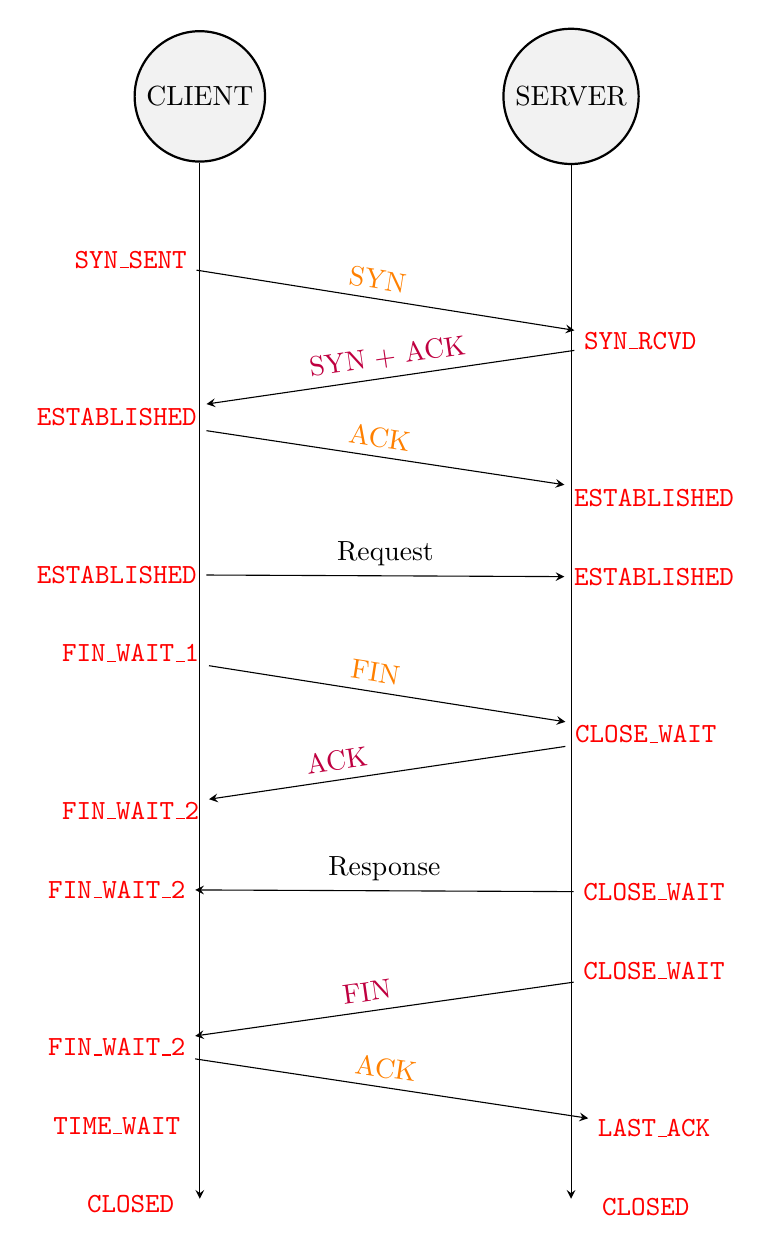
\begin{tikzpicture}
			\node[state] (CLIENT) {CLIENT};
			\node[state, right=of CLIENT] (SERVER) {SERVER};
			\node[below=1cm of CLIENT, xshift=-25] (t0) {\textcolor{red}{$\texttt{SYN\_SENT}$}};
			\node[below=2cm of SERVER, xshift=25] (t1) {\textcolor{red}{$\texttt{SYN\_RCVD}$}};
			\node[below=3cm of CLIENT, xshift=-30] (t2) {\textcolor{red}{$\texttt{ESTABLISHED}$}};
			\node[below=4cm of SERVER, xshift=30] (t3) {\textcolor{red}{$\texttt{ESTABLISHED}$}};
			\node[below=5cm of CLIENT, xshift=-30] (t4) {\textcolor{red}{$\texttt{ESTABLISHED}$}};
			\node[below=5cm of SERVER, xshift=30] (t5) {\textcolor{red}{$\texttt{ESTABLISHED}$}};
			\node[below=6cm of CLIENT, xshift=-25] (t6) {\textcolor{red}{$\texttt{FIN\_WAIT\_1}$}};
			\node[below=7cm of SERVER,xshift=27] (t7) {\textcolor{red}{$\texttt{CLOSE\_WAIT}$}};
			\node[below=8cm of CLIENT, xshift=-25] (t8) {\textcolor{red}{$\texttt{FIN\_WAIT\_2}$}};
			\node[below=9cm of CLIENT, xshift=-30] (t9) {\textcolor{red}{$\texttt{FIN\_WAIT\_2}$}};
			\node[below=9cm of SERVER, xshift=30] (t10) {\textcolor{red}{$\texttt{CLOSE\_WAIT}$}};
			\node[below=10cm of SERVER, xshift=30] (t12) {\textcolor{red}{$\texttt{CLOSE\_WAIT}$}};
			\node[below=11cm of CLIENT, xshift=-30] (t11) {\textcolor{red}{$\texttt{FIN\_WAIT\_2}$}};
			\node[below=12cm of SERVER, xshift=30] (t13) {\textcolor{red}{$\texttt{LAST\_ACK}$}};
			\node[below=12cm of CLIENT, xshift=-30] (wait) {\textcolor{red}{$\texttt{TIME\_WAIT}$}};
			\node[below=13cm of CLIENT, xshift=-25] (t14) {\textcolor{red}{$\texttt{CLOSED}$}};
			\node[below=13cm of SERVER,xshift=27] (t15) {\textcolor{red}{$\texttt{CLOSED}$}};
			
			
			\draw (CLIENT) -- ++(0,-14cm);
			\draw (SERVER) -- ++(0, -14cm);
			\draw (t0) edge[] node[pos=0.5, sloped, above]{\parbox{1cm}{\textcolor{orange}{SYN}}} (t1);
			\draw (t1) edge[] node[pos=0.5, sloped, above]{\parbox{2cm}{\textcolor{purple}{SYN + ACK}}} (t2);
			\draw (t2) edge[] node[pos=0.5, sloped, above]{\parbox{1cm}{\textcolor{orange}{ACK}}} (t3);
			\draw (t4) edge[] node[above]{Request} (t5);
			\draw  (t6) edge[] node[pos=0.5, sloped, above]{\parbox{1cm}{\textcolor{orange}{FIN}}} (t7);
			\draw  (t7) edge[] node[pos=0.5, sloped, above]{\parbox{2cm}{\textcolor{purple}{ACK}}} (t8);
			\draw (t10) edge[] node[above]{Response} (t9);
			\draw  (t12) edge[] node[pos=0.5, sloped, above]{\parbox{1cm}{\textcolor{purple}{FIN}}} (t11);
			\draw  (t11) edge[] node[pos=0.5, sloped, above]{\parbox{1cm}{\textcolor{orange}{ACK}}} (t13);
		\end{tikzpicture}
	\end{figure}
	
	\section{Scenario 3}
	
	\begin{tcolorbox}
		Simultaneous connect.
	\end{tcolorbox}
	
	\begin{figure}[h]
		\centering
		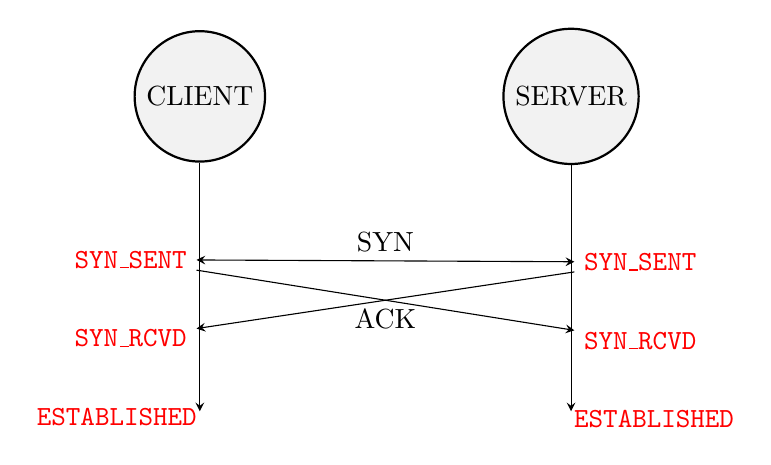
\begin{tikzpicture}
			\node[state] (CLIENT) {CLIENT};
			\node[state, right=of CLIENT] (SERVER) {SERVER};
			\node[below=1cm of CLIENT, xshift=-25] (t0) {\textcolor{red}{$\texttt{SYN\_SENT}$}};
			\node[below=1cm of SERVER, xshift=25] (t1) {\textcolor{red}{$\texttt{SYN\_SENT}$}};
			\node[below=2cm of CLIENT, xshift=-25] (t2) {\textcolor{red}{$\texttt{SYN\_RCVD}$}};
			\node[below=2cm of SERVER, xshift=25] (t3) {\textcolor{red}{$\texttt{SYN\_RCVD}$}};
			\node[below=3cm of CLIENT, xshift=-30] (t4) {\textcolor{red}{$\texttt{ESTABLISHED}$}};
			\node[below=3cm of SERVER, xshift=30] (t5) {\textcolor{red}{$\texttt{ESTABLISHED}$}};
			
			
			\draw (CLIENT) -- ++(0, -4cm);
			\draw (SERVER) -- ++(0, -4cm);
			\draw[<->] (t0) edge[] node[above]{SYN} (t1);
			\draw (t0) edge[] node[below]{ACK} (t3);
			\draw (t1) edge[] node[]{} (t2);
		\end{tikzpicture}
	\end{figure}
	
	\section{Scenario 4}
	
	\begin{tcolorbox}
		Simultaneous close.
	\end{tcolorbox}
	
	\begin{figure}[h]
		\centering
		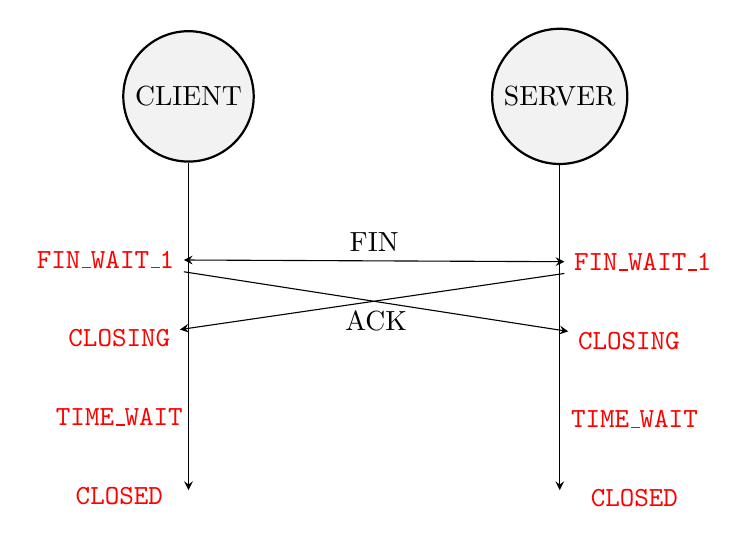
\begin{tikzpicture}
			\node[state] (CLIENT) {CLIENT};
			\node[state, right=of CLIENT] (SERVER) {SERVER};
			\node[below=1cm of CLIENT, xshift=-30] (t0) {\textcolor{red}{$\texttt{FIN\_WAIT\_1}$}};
			\node[below=1cm of SERVER, xshift=30] (t1) {\textcolor{red}{$\texttt{FIN\_WAIT\_1}$}};
			\node[below=2cm of CLIENT, xshift=-25] (t2) {\textcolor{red}{$\texttt{CLOSING}$}};
			\node[below=2cm of SERVER, xshift=25] (t3) {\textcolor{red}{$\texttt{CLOSING}$}};
			\node[below=3cm of CLIENT, xshift=-25] (t14) {\textcolor{red}{$\texttt{TIME\_WAIT}$}};
			\node[below=3cm of SERVER,xshift=27] (t15) {\textcolor{red}{$\texttt{TIME\_WAIT}$}};
			\node[below=4cm of CLIENT, xshift=-25] (t14) {\textcolor{red}{$\texttt{CLOSED}$}};
			\node[below=4cm of SERVER,xshift=27] (t15) {\textcolor{red}{$\texttt{CLOSED}$}};
			
			
			\draw (CLIENT) -- ++(0, -5cm);
			\draw (SERVER) -- ++(0, -5cm);
			\draw[<->] (t0) edge[] node[above]{FIN} (t1);
			\draw (t0) edge[] node[below]{ACK} (t3);
			\draw (t1) edge[] node[]{} (t2);
		\end{tikzpicture}
	\end{figure}
	
	\section{Scenario 5}
	
	\begin{tcolorbox}
		A client connects to a server. The server is only ever able to receive data, never send it, and therefore immediately brings the connection into half-closed state (closed in the direction server $\to$ client).
	\end{tcolorbox}
	
	\begin{figure}[h]
		\centering
		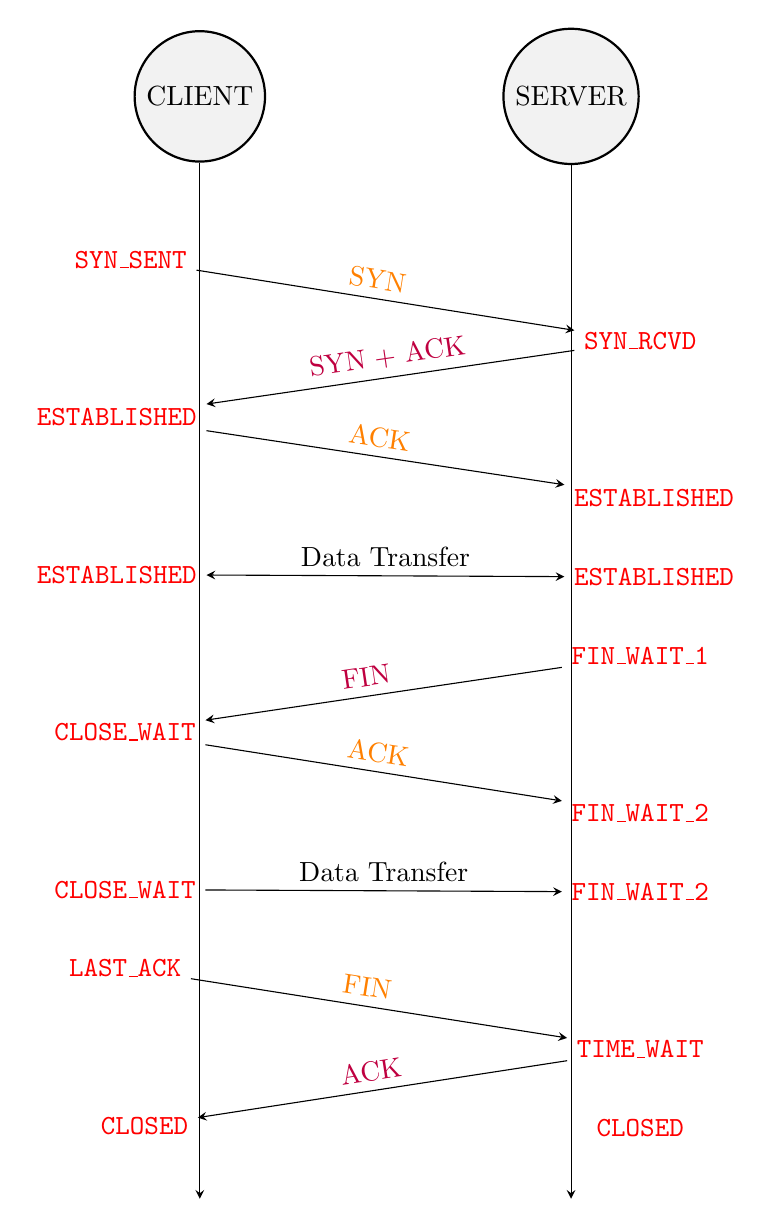
\begin{tikzpicture}
			\node[state] (CLIENT) {CLIENT};
			\node[state, right=of CLIENT] (SERVER) {SERVER};
			\node[below=1cm of CLIENT, xshift=-25] (t0) {\textcolor{red}{$\texttt{SYN\_SENT}$}};
			\node[below=2cm of SERVER, xshift=25] (t1) {\textcolor{red}{$\texttt{SYN\_RCVD}$}};
			\node[below=3cm of CLIENT, xshift=-30] (t2) {\textcolor{red}{$\texttt{ESTABLISHED}$}};
			\node[below=4cm of SERVER, xshift=30] (t3) {\textcolor{red}{$\texttt{ESTABLISHED}$}};
			\node[below=5cm of CLIENT, xshift=-30] (t4) {\textcolor{red}{$\texttt{ESTABLISHED}$}};
			\node[below=5cm of SERVER, xshift=30] (t5) {\textcolor{red}{$\texttt{ESTABLISHED}$}};
			\node[below=6cm of SERVER, xshift=25] (t6) {\textcolor{red}{$\texttt{FIN\_WAIT\_1}$}};
			\node[below=7cm of CLIENT,xshift=-27] (t7) {\textcolor{red}{$\texttt{CLOSE\_WAIT}$}};
			\node[below=8cm of SERVER, xshift=25] (t8) {\textcolor{red}{$\texttt{FIN\_WAIT\_2}$}};
			\node[below=9cm of CLIENT,xshift=-27] (t9) {\textcolor{red}{$\texttt{CLOSE\_WAIT}$}};
			\node[below=9cm of SERVER, xshift=25] (t10) {\textcolor{red}{$\texttt{FIN\_WAIT\_2}$}};
			\node[below=10cm of CLIENT,xshift=-27] (t11) {\textcolor{red}{$\texttt{LAST\_ACK}$}};
			\node[below=11cm of SERVER, xshift=25] (t12) {\textcolor{red}{$\texttt{TIME\_WAIT}$}};
			\node[below=12cm of CLIENT, xshift=-20] (t13) {\textcolor{red}{$\texttt{CLOSED}$}};
			\node[below=12cm of SERVER, xshift=25] (t14) {\textcolor{red}{$\texttt{CLOSED}$}};
			
			
			
			\draw (CLIENT) -- ++(0, -14cm);
			\draw (SERVER) -- ++(0, -14cm);
			\draw (t0) edge[] node[pos=0.5, sloped, above]{\parbox{1cm}{\textcolor{orange}{SYN}}} (t1);
			\draw (t1) edge[] node[pos=0.5, sloped, above]{\parbox{2cm}{\textcolor{purple}{SYN + ACK}}} (t2);
			\draw (t2) edge[] node[pos=0.5, sloped, above]{\parbox{1cm}{\textcolor{orange}{ACK}}} (t3);
			\draw[<->] (t4) edge[] node[above]{Data Transfer} (t5);
			\draw  (t6) edge[] node[pos=0.5, sloped, above]{\parbox{1cm}{\textcolor{purple}{FIN}}} (t7);
			\draw  (t7) edge[] node[pos=0.5, sloped, above]{\parbox{1cm}{\textcolor{orange}{ACK}}} (t8);
			\draw  (t9) edge[] node[above]{Data Transfer} (t10);
			\draw  (t11) edge[] node[pos=0.5, sloped, above]{\parbox{1cm}{\textcolor{orange}{FIN}}} (t12);
			\draw  (t12) edge[] node[pos=0.5, sloped, above]{\parbox{1cm}{\textcolor{purple}{ACK}}} (t13);
			
		\end{tikzpicture}
	\end{figure}
	
\end{document}